\documentclass[a4paper,11pt]{article}

\usepackage[portuguese]{babel}
\usepackage[utf8]{inputenc}
\usepackage{amsmath}
\usepackage{graphicx}
\usepackage{hyperref}
\usepackage{float}
\usepackage{subfig}
\usepackage{fixltx2e}
\usepackage[bottom]{footmisc}
\usepackage{listings}
\usepackage{xargs}                      % Use more than one optional parameter in a new commands
\usepackage[pdftex,dvipsnames]{xcolor}  % Coloured text etc.
\usepackage[colorinlistoftodos,prependcaption,textsize=tiny]{todonotes}
\newcommandx{\unsure}[2][1=]{\todo[linecolor=red,backgroundcolor=red!25,bordercolor=red,#1]{#2}}
\newcommandx{\change}[2][1=]{\todo[linecolor=blue,backgroundcolor=blue!25,bordercolor=blue,#1]{#2}}
\newcommandx{\info}[2][1=]{\todo[linecolor=OliveGreen,backgroundcolor=OliveGreen!25,bordercolor=OliveGreen,#1]{#2}}
\newcommandx{\improvement}[2][1=]{\todo[linecolor=Plum,backgroundcolor=Plum!25,bordercolor=Plum,#1]{#2}}
\newcommandx{\thiswillnotshow}[2][1=]{\todo[disable,#1]{#2}}
\usepackage[font=footnotesize]{caption}
\usepackage[hypcap]{caption}
\usepackage[top=2.5cm, bottom=2.5cm, left=2.5cm, right=2.5cm]{geometry}
\usepackage{enumerate}

\setcounter{tocdepth}{2}

\numberwithin{equation}{section}
\addto\captionsportuguese{\renewcommand{\contentsname}{Índice}}

\linespread{1.3}
\usepackage{indentfirst}

\begin{document}
\begin{titlepage}
\begin{center}

\hfill \break
\hfill \break


\includegraphics[width=0.3\textwidth]{img/logo}~\\[1cm] 

\textsc{\LARGE Instituto Superior Técnico}\\[0.25cm]
\textsc{\Large Mestrado Integrado em Engenharia Electrotécnica e de Computadores}\\[1.8cm]
\textsc{\huge Electrónica de Potência}\\[0.25cm]

\vspace{6mm}

{\huge \bfseries Circuito de Disparo de um Tiristor \linebreak \& \linebreak Circuito com Carga Ressonante \linebreak Comutação pela Carga  \\[1cm]}

\begin{tabular}{ l l }
	João Bernardo Sequeira de Sá & \hspace{2mm} n.º 68254 \\
	Maria Margarida Dias dos Reis & \hspace{2mm} n.º 73099 \\
	Rafael Augusto Maleno Charrama Gonçalves & \hspace{2mm} n.º 73786 \\
	Nuno Miguel Rodrigues Machado & \hspace{2mm} n.º 74236
\end{tabular}

\vspace{7mm}

Grupo n.º TAL de segunda-feira das 17h00 - 2000

\vfill

{\large Lisboa, 12 de Outubro de 2015} 
	
\end{center}
\end{titlepage}
	
\tableofcontents
\pagebreak

\section{Introdução}

Pretende-se com este trabalho estudar o comportamento do tiristor, com especial interesse na passagem à condução e ao corte deste dispositivo, assim como evidenciar alguns aspetos da sua utilização em circuitos de conversão de potência.

O tiristor, ou retificador controlado de silício, é o dispositivo indicado para comandar tensões e correntes de valor elevado, sendo capaz de suportar potências da ordem dos 10 MW. É composto por três terminais, o elétrodo de disparo, ou \textit{gate} (G), ânodo (A) e cátodo (K). Através da \textit{gate} pode levar-se o dispositivo à condução, caso este esteja polarizado diretamente nos terminais de ânodo e cátodo, através de um impulso. 

Por norma, os terminais de potência, ânodo e cátodo, desempenham funções semelhantes aos terminais do díodo. Em oposição ao transístor, o tiristor é um dispositivo que possui memória; uma vez que seja colocado à condução não regressa ao estado de bloqueio através de atuação na gate, mas sim através de um anulamento da corrente, polarização inversa, comportamento idêntico ao do díodo. Gera-se assim uma necessidade para que, caso o circuito em que o dispositivo é aplicado não possua uma comutação natural, se recorra a técnicas de comutação forçada.

Estas técnicas de comutação forçada são concebidas normalmente com recurso a componentes reativos, como sejam a bobine ou o condensador, para que possa ser estabelecida uma polarização inversa aos terminais do tiristor num certo período de tempo do funcionamento do circuito. Estas técnicas levam no entanto a perdas, pelo que as frequências de operação são da ordem de 500 a 1.5 kHz.

Atualmente existe tendência para usar como alternativa IGBT's ou GTO's.

\pagebreak

\section{Circuito de Disparo}

\subsection{Funcionamento}

De forma a estudar o comportamento de circuitos com semicondutores de potência é necessário, em primeira instância, realizar o circuito de “drive” ou ataque ao terminal de controlo ou, no caso de tiristores, o circuito de disparo. Este circuito tem a função de estabelecer o sinal de comando do tiristor, sendo este aplicado entre a \textit{gate} e o cátodo, assim como estabelecer o isolamento galvânico entre o circuito de potência e o circuito de controlo. Pode observar-se este circuito na \autoref{fig:circuit_1}.

\begin{figure}[h]
	\centering
	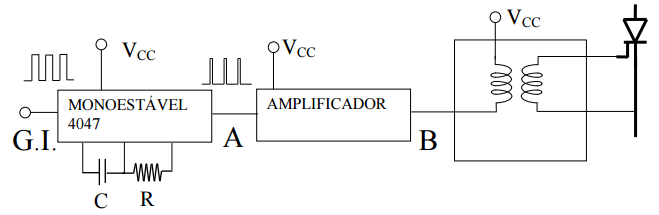
\includegraphics[keepaspectratio=true, scale=0.37]{teoricas/trigger_circuit}
	\caption{Circuito de disparo.}
	\label{fig:circuit_1}
	\vspace{-0.8em}
\end{figure}

O objetivo neste trabalho é assim realizar este circuito com uma frequência de 2 kHz, fazendo para isso uso de um sinal com esta frequência originado por um gerador de impulsos (GI). O circuito de disparo será então composto por uma monoestável que reage ao flanco ascendente do sinal originado pelo GI; tem-se assim à saída da monoestável um impulso cuja duração será função da resistência $R$ e condensador $C$. 

A duração deste impulso deve ser definida consoante as características da \textit{gate} do tiristor que se está a utilizar, sendo neste caso de 10 $\mu$s. Este impulso tem, no entanto, que ser amplificado para que seja injetada corrente suficiente na \textit{gate} do tiristor. Usa-se assim um transístor de ganho elevado, transitando da saturação ao corte, estabelecendo uma tensão no primário do transformador, sempre que surja o impulso na saída da monoestável. As formas de onda destes impulsos podem ser observadas na \autoref{fig:circuit_2}.

\begin{figure}[h]
	\centering
	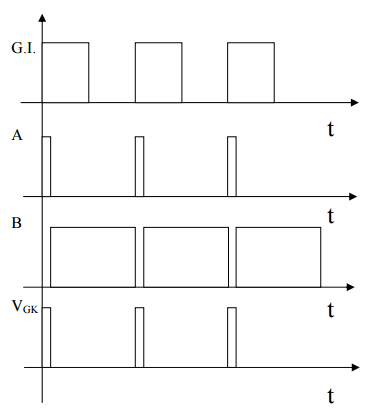
\includegraphics[keepaspectratio=true, scale=0.45]{teoricas/trigger_waveform}
	\caption{Formas de onda das tensões no circuito de disparo.}
	\label{fig:circuit_2}
	\vspace{-0.8em}
\end{figure}

O transformador serve também para que se obtenha o isolamento galvânico entre os circuitos de disparo e de potência.

\subsection{Montagem e equipamento}

A montagem presente na placa impressa utilizada no laboratório pode ser observada na \autoref{fig:circuit_3}.

\begin{figure}[h]
	\centering
	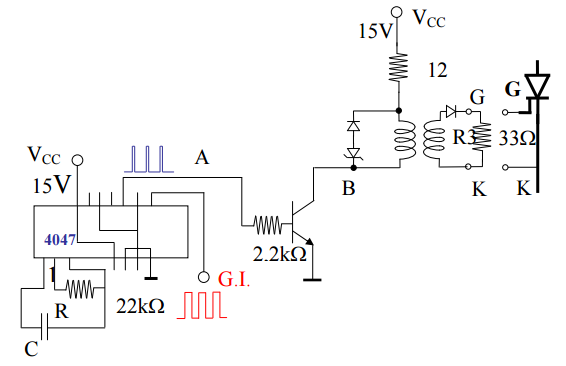
\includegraphics[keepaspectratio=true, scale=0.45]{teoricas/assembly_circuit}
	\caption{Esquema elétrico do circuito de disparo presente na placa impressa.}
	\label{fig:circuit_3}
	\vspace{-0.8em}
\end{figure}

Tal como dito na secção acima, a duração do impulso, $T$, será definida pela resistência $R$ e o condensador $C$ segundo a seguinte fórmula dada pelo fabricante.

\vspace{-3mm}
\begin{equation}
T = 2.88 \ RC.
\end{equation}

Para que se tenha 10 $\mu$s faz-se assim uso de uma resistência com $10$ k$\Omega$ e $0.4$ nF, sem necessidade de uma grande precisão nos valores, pois a exatidão do tempo de disparo neste circuito não é prevalente.

O equipamento a utilizar na condução do trabalho é assim:

\vspace{-2mm}

\begin{itemize}
	\item 1 osciloscópio;
	\vspace{-2mm}	
	\item 1 sonda de corrente;
	\vspace{-2mm}	
	\item 1 gerador de impulsos;
	\vspace{-2mm}	
	\item 2 fontes de alimentação;
	\vspace{-2mm}	
	\item 2 multímetros;
	\vspace{-2mm}	
	\item 1 placa de circuito impresso.
\end{itemize}

\pagebreak

\section{Condução do Trabalho}

\subsection{Estudo do circuito de disparo}

Em primeira instância apenas se realizam as ligações do circuito de disparo à fonte de alimentação. Após as ligações feitas sintoniza-se o GI para que se obtenha na saída uma onda retangular de amplitude $0$ a $15$ a uma frequência de $2$ kHz.

\subsubsection{Formas de onda da tensão entre o ponto A e a massa e entre o ponto B e a massa}

Feito isto, podem observar-se as formas de onda entre o ponto A e a massa e o ponto B e a massa no osciloscópio tal como na \autoref{fig:photo 1}.

\begin{figure}[h]
	\centering
	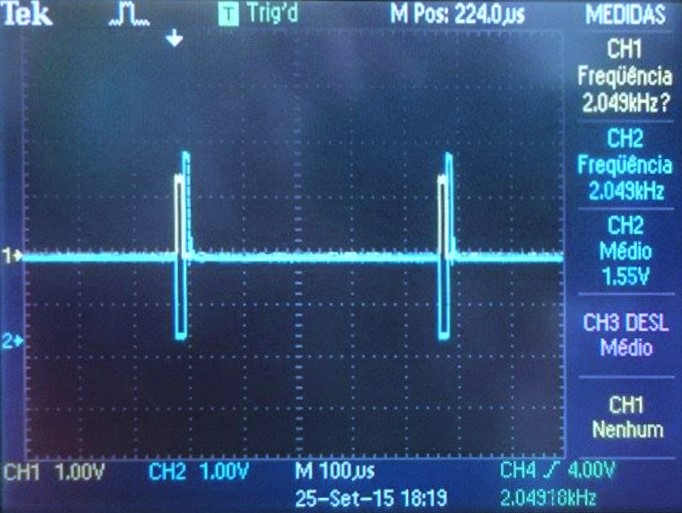
\includegraphics[keepaspectratio=true, scale=0.55]{img/fig4}
	\caption{Tensões nos pontos A (a amarelo) e B (a azul).}
	\label{fig:photo 1}
	\vspace{-0.8em}
\end{figure}

Tem-se assim no canal $1$ (amarelo) a tensão no ponto A e no canal $2$ (azul) a tensão no ponto B. Para o canal 1 observa-se uma onda quadrada compreendida entre 0 e 14,8 V, frequência de $2$ kHz, duração de impulso de $13$ $\mu$s e um fator de ciclo de 2,6\%. O canal $2$ apresenta uma onda retangular com $1,5$ V no qual existe um pico de tensão no flanco ascendente com $3,4$ V estabilizando ao fim de aproximadamente $15$ $\mu$s. A duração do sinal retangular no canal 2 é de aproximadamente 470 $\mu$s o que leva a um fator de ciclo de 94\%.

Na \autoref{fig:photo 2} fez-se \textit{zoom} de forma a que o pico de tensão da onda retangular no canal 2 se possa observar melhor, assim como a relação entre as tensões em A e B.

\pagebreak

\begin{figure}[h]
	\centering
	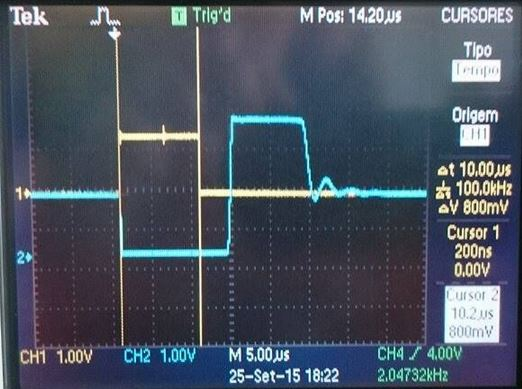
\includegraphics[keepaspectratio=true, scale=0.6]{img/fig5}
	\caption{\textit{Zoom} das tensões nos pontos A e B.}
	\label{fig:photo 2}
	\vspace{-0.8em}
\end{figure}

Este pico deve-se a que, no momento em que o transístor entra em condução, a bobina encontra-se magnetizada ficando os díodos diretamente polarizados, sendo que a tensão em B será a soma entre a tensão no primário do transformador e VCC. Após o período de desmagnetização esta estabiliza no valor devido, VCC. 

Existe também um atraso apreciável entre a tensão em A e B que se deve ao tempo de passagem do transístor da saturação para o corte.

\subsubsection{Díodos no primário do transformador}

Considera-se agora relevante enunciar a funcionalidade dos díodos presentes no circuito. Em primeiro tem-se o díodo ligado ao primário do transformador cuja função é essencialmente garantir a continuidade da corrente quando o transístor passa ao corte, ficando assim a bobina salvaguardada de potenciais descontinuidades na corrente (o que é essencial uma vez que, na bobina, a corrente é variável de estado), garantindo o bom funcionamento do circuito. 

Tem-se ainda o díodo Zenner cujo objetivo é diminuir o tempo de desmagnetização da bobina. Isto é devido à superior tensão imposta por este díodo aos terminais do transformador (tensão de Zenner), elevando assim a corrente que ali circula. A circulação de corrente pelos díodos acontece até que haja a total desmagnetização da
bobina.

\subsubsection{Tensão no primário do transformador em função do díodo Zenner}

A alteração provocada pelo díodo Zenner no comportamento do circuito é evidenciada na \autoref{fig:photo 3} e \autoref{fig:photo 4}.

\pagebreak

\begin{figure}[h]
	\centering
	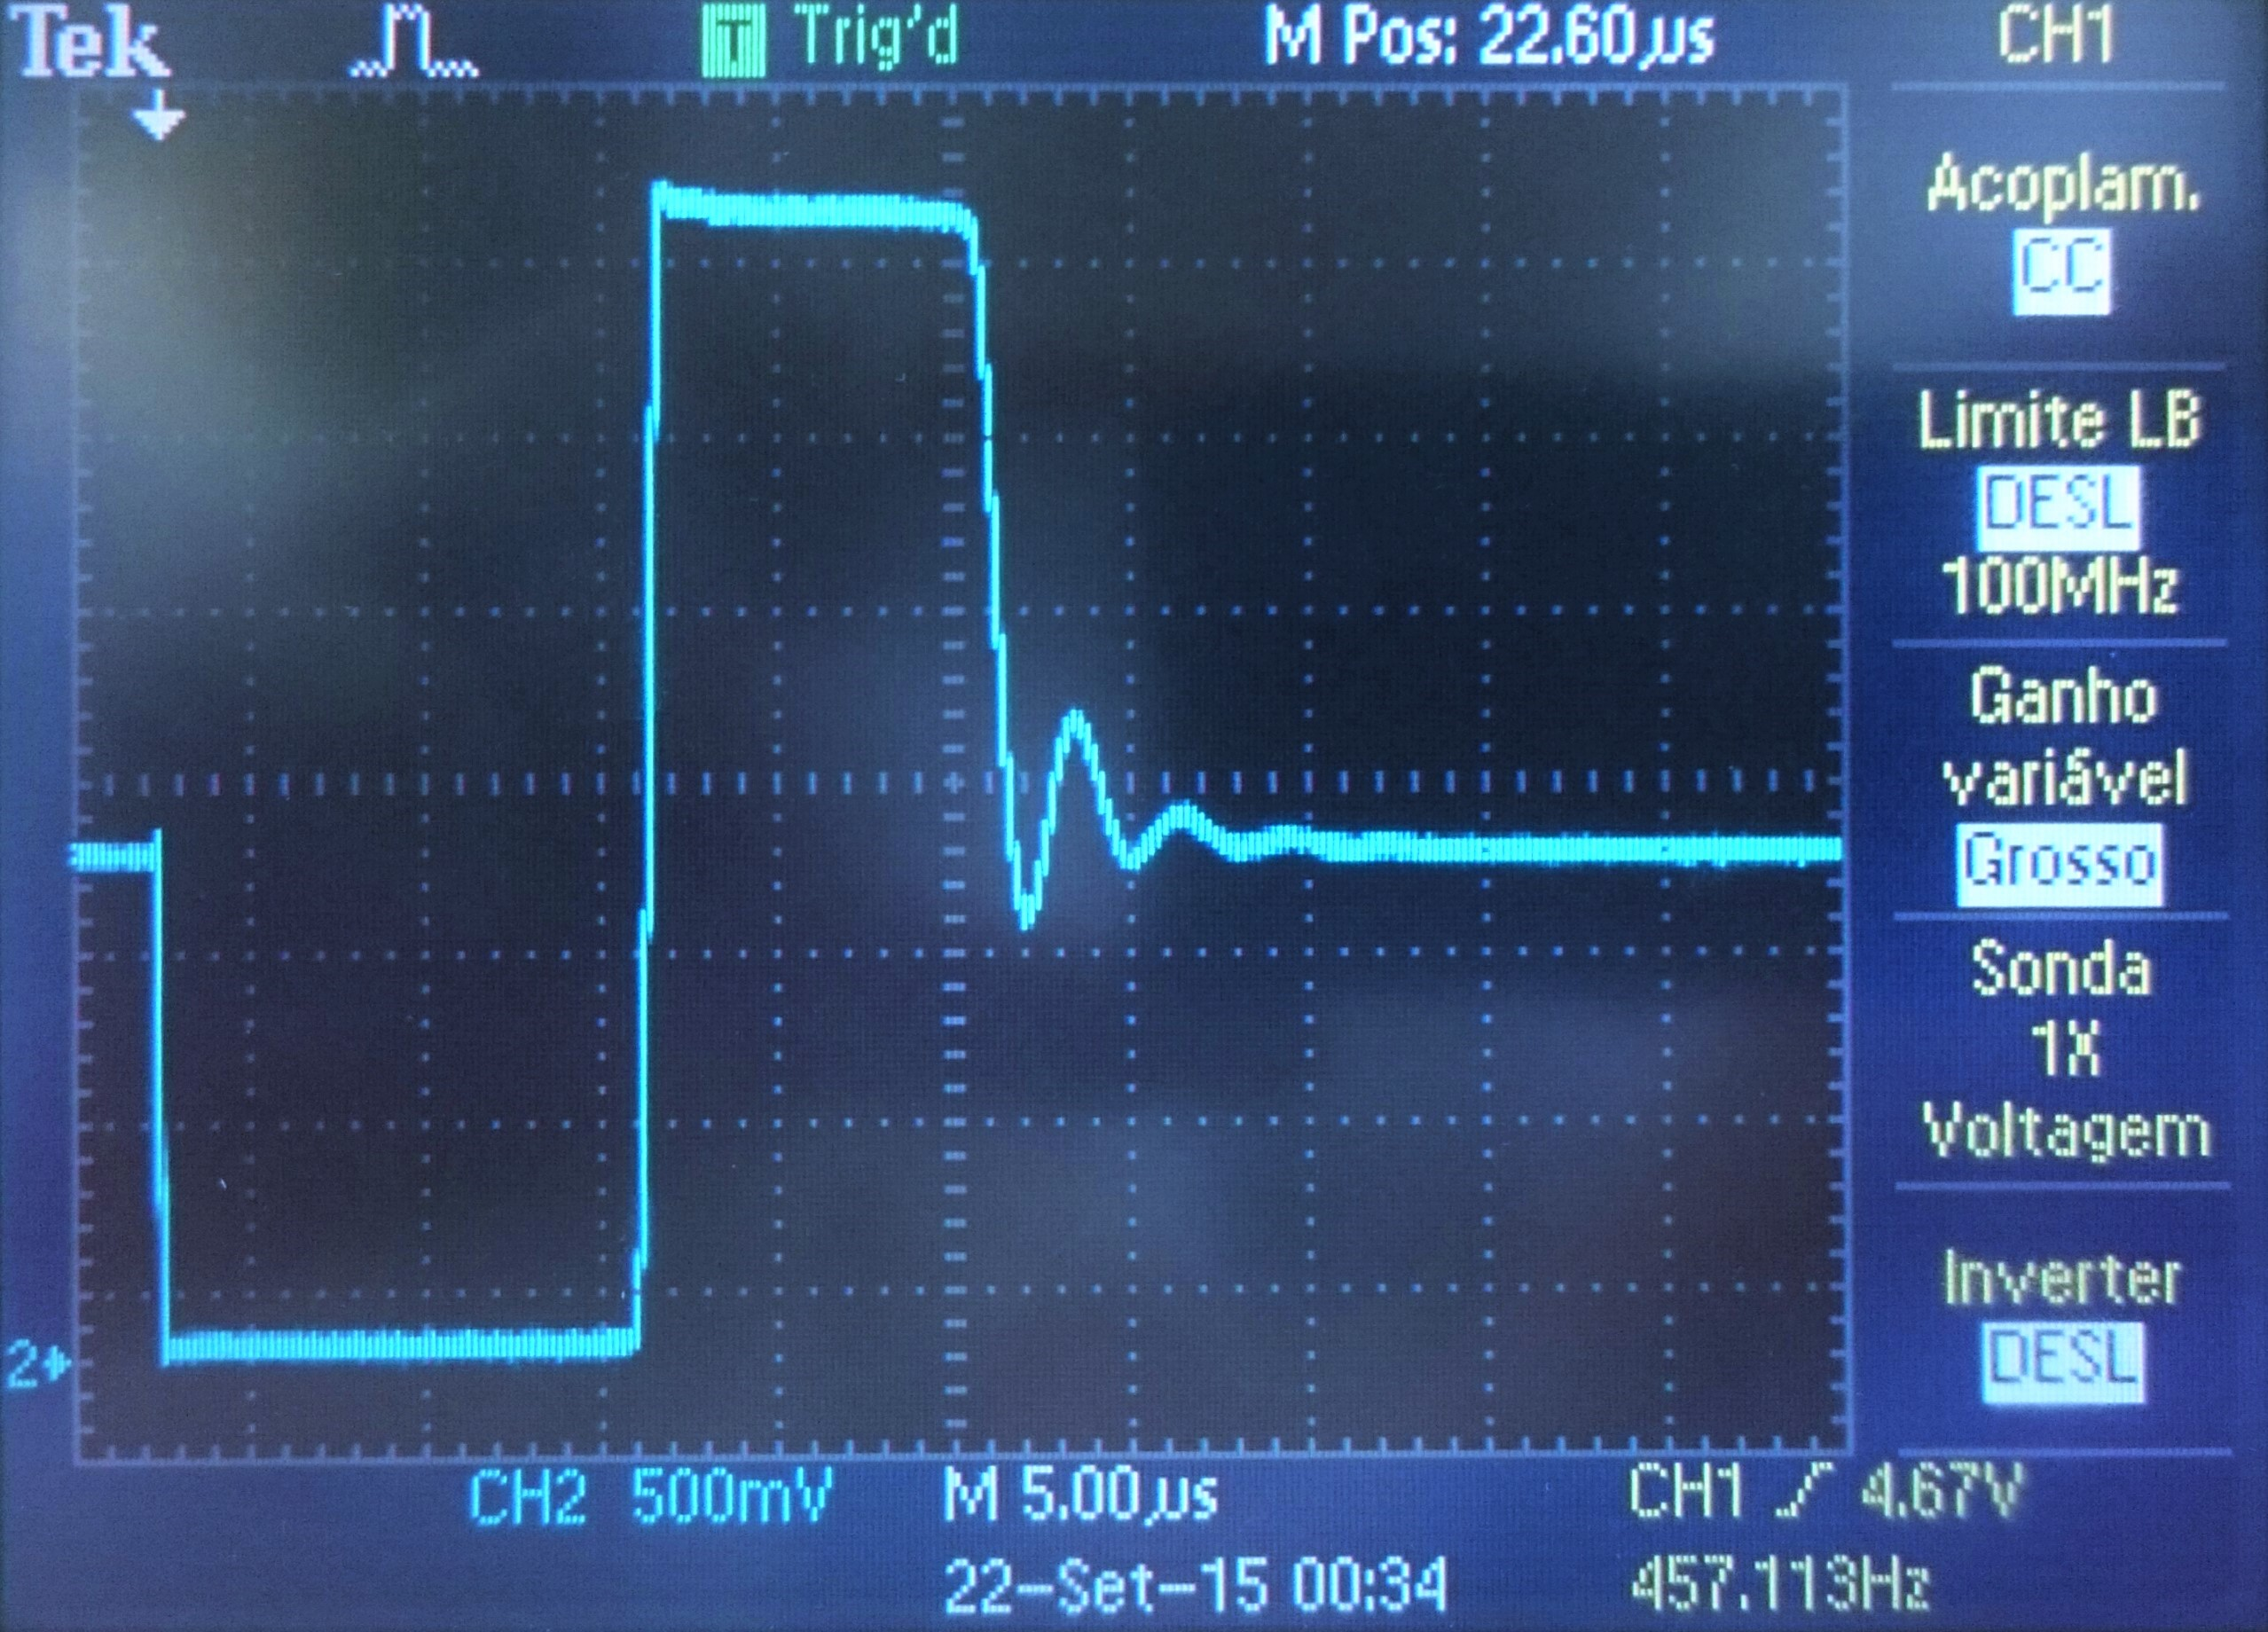
\includegraphics[keepaspectratio=true, scale=0.15]{img/DSC0118}
	\caption{Tensão no ponto B com o díodo Zenner.}
	\label{fig:photo 3}
	\vspace{-0.8em}
\end{figure}

\begin{figure}[h]
	\vspace{3mm}
	\centering
	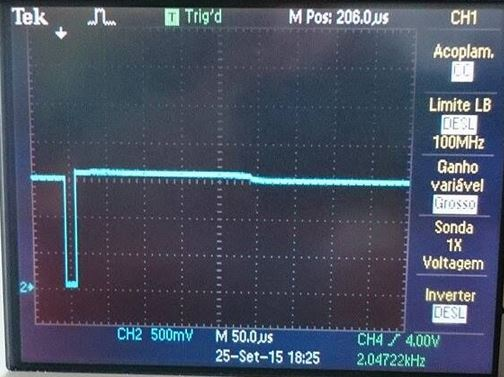
\includegraphics[keepaspectratio=true, scale=0.63]{img/fig7}
	\caption{Tensão no ponto B sem o díodo Zenner.}
	\label{fig:photo 4}
	\vspace{-0.8em}
\end{figure}

Na \autoref{fig:photo 3} pode concluir-se que o tempo de desmagnetização é relativamente curto, cerca de $30$ $\mu$s em oposição ao tempo de desmagnetização observável na \autoref{fig:photo 4}, onde será aproximadamente $225$ $\mu$s, valor muito superior ao caso em que se faz uso do díodo Zenner.

O díodo Zenner conduz quando inversamente polarizado (neste caso, a tensão de Zenner é de $-17$ V), o que leva a uma dissipação muito mais rápida, e consequentemente acelera o processo de desmagnetização. Verifica-se que, em ambos os casos, a área da curva de magnetização é idêntica à área da curva de desmagnetização. Sem díodo Zenner, o valor da curva de desmagnetização é mais baixo, pelo que leva mais tempo a satisfazer este requisito. 

\subsubsection{Tensão entre a \textit{gate} e o cátodo do tiristor}

Seguidamente visualizou-se a tensão aos terminais da resistência R\textsubscript{3},  V\textsubscript{GK} tal como se tem na \autoref{fig:photo 5}.

\begin{figure}[h]
	\centering
	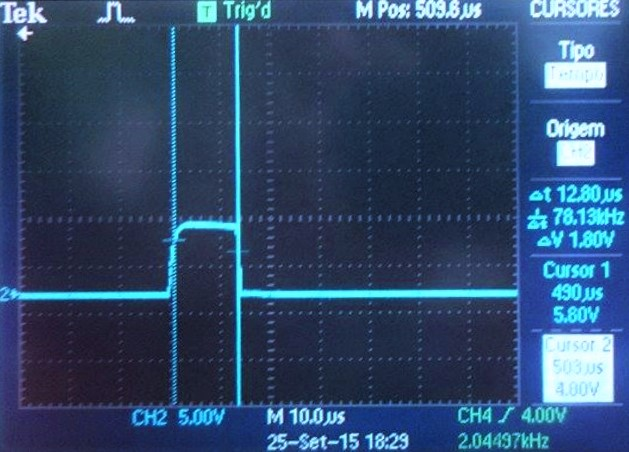
\includegraphics[keepaspectratio=true, scale=0.63]{img/fig8}
	\caption{Tensão V\textsubscript{GK} na resistência R\textsubscript{3}.}
	\label{fig:photo 5}
	\vspace{-0.8em}
\end{figure}

Trata-se portanto de um sinal retangular com duração de impulso de 13 $\mu$s, amplitude de aproximadamente 8 V e um fator de ciclo de 2,6\% que são as características necessárias para se ter o sinal de comando do tiristor.

De forma a que a primeira parte do trabalho esteja concluída passou-se a desligar os terminais da resistência, seguido da realização das ligação dos pontos G e K à \textit{gate} e cátodo do tiristor, respetivamente.

\subsection{Estudo do circuito de potência}

Pretende-se agora verificar, como já foi referido, que o tiristor é um dispositivo que, por si só, não tem a capacidade de cortar a corrente que conduz. Assim, efetuam-se duas montagens distintas, tal como se tem na \autoref{fig:teorica1}.

\begin{figure}[H]
	\centering
	\subfloat[]{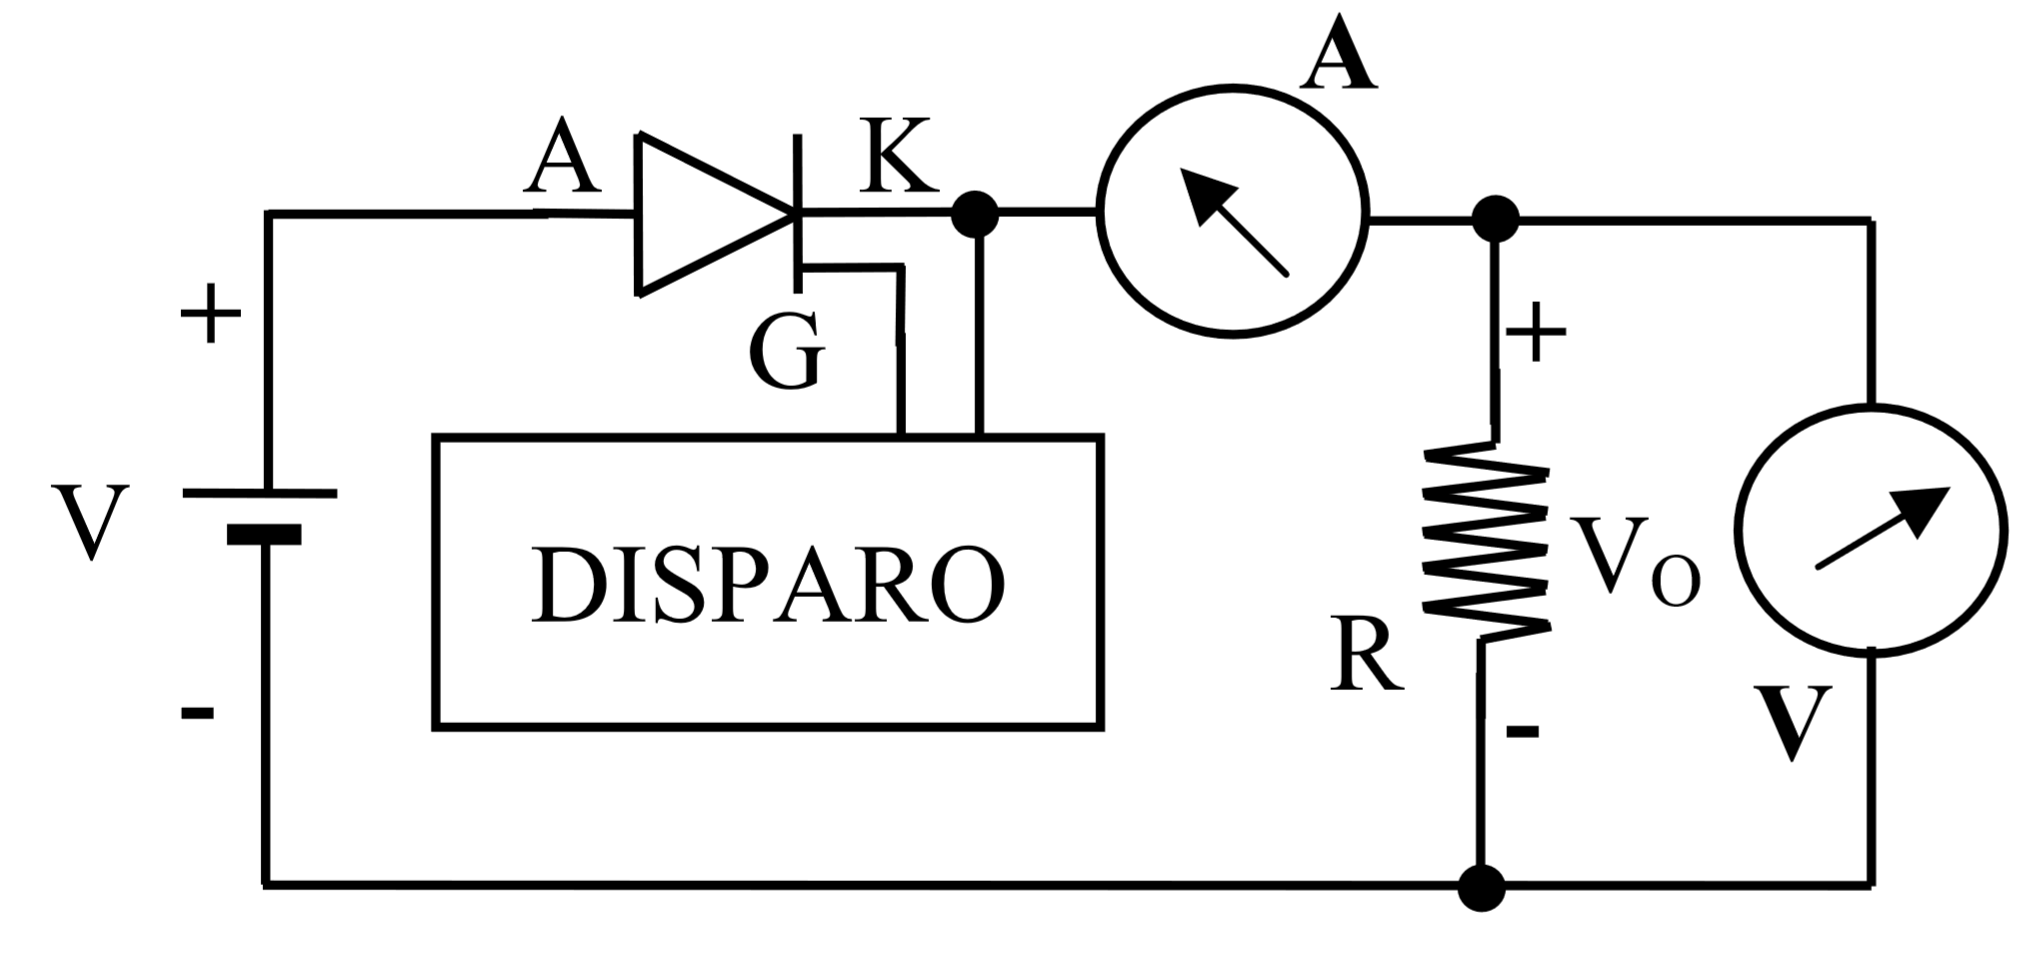
\includegraphics[keepaspectratio=true, scale=0.17]{teoricas/no_cut}}
	\hspace{8mm}
	\subfloat[]{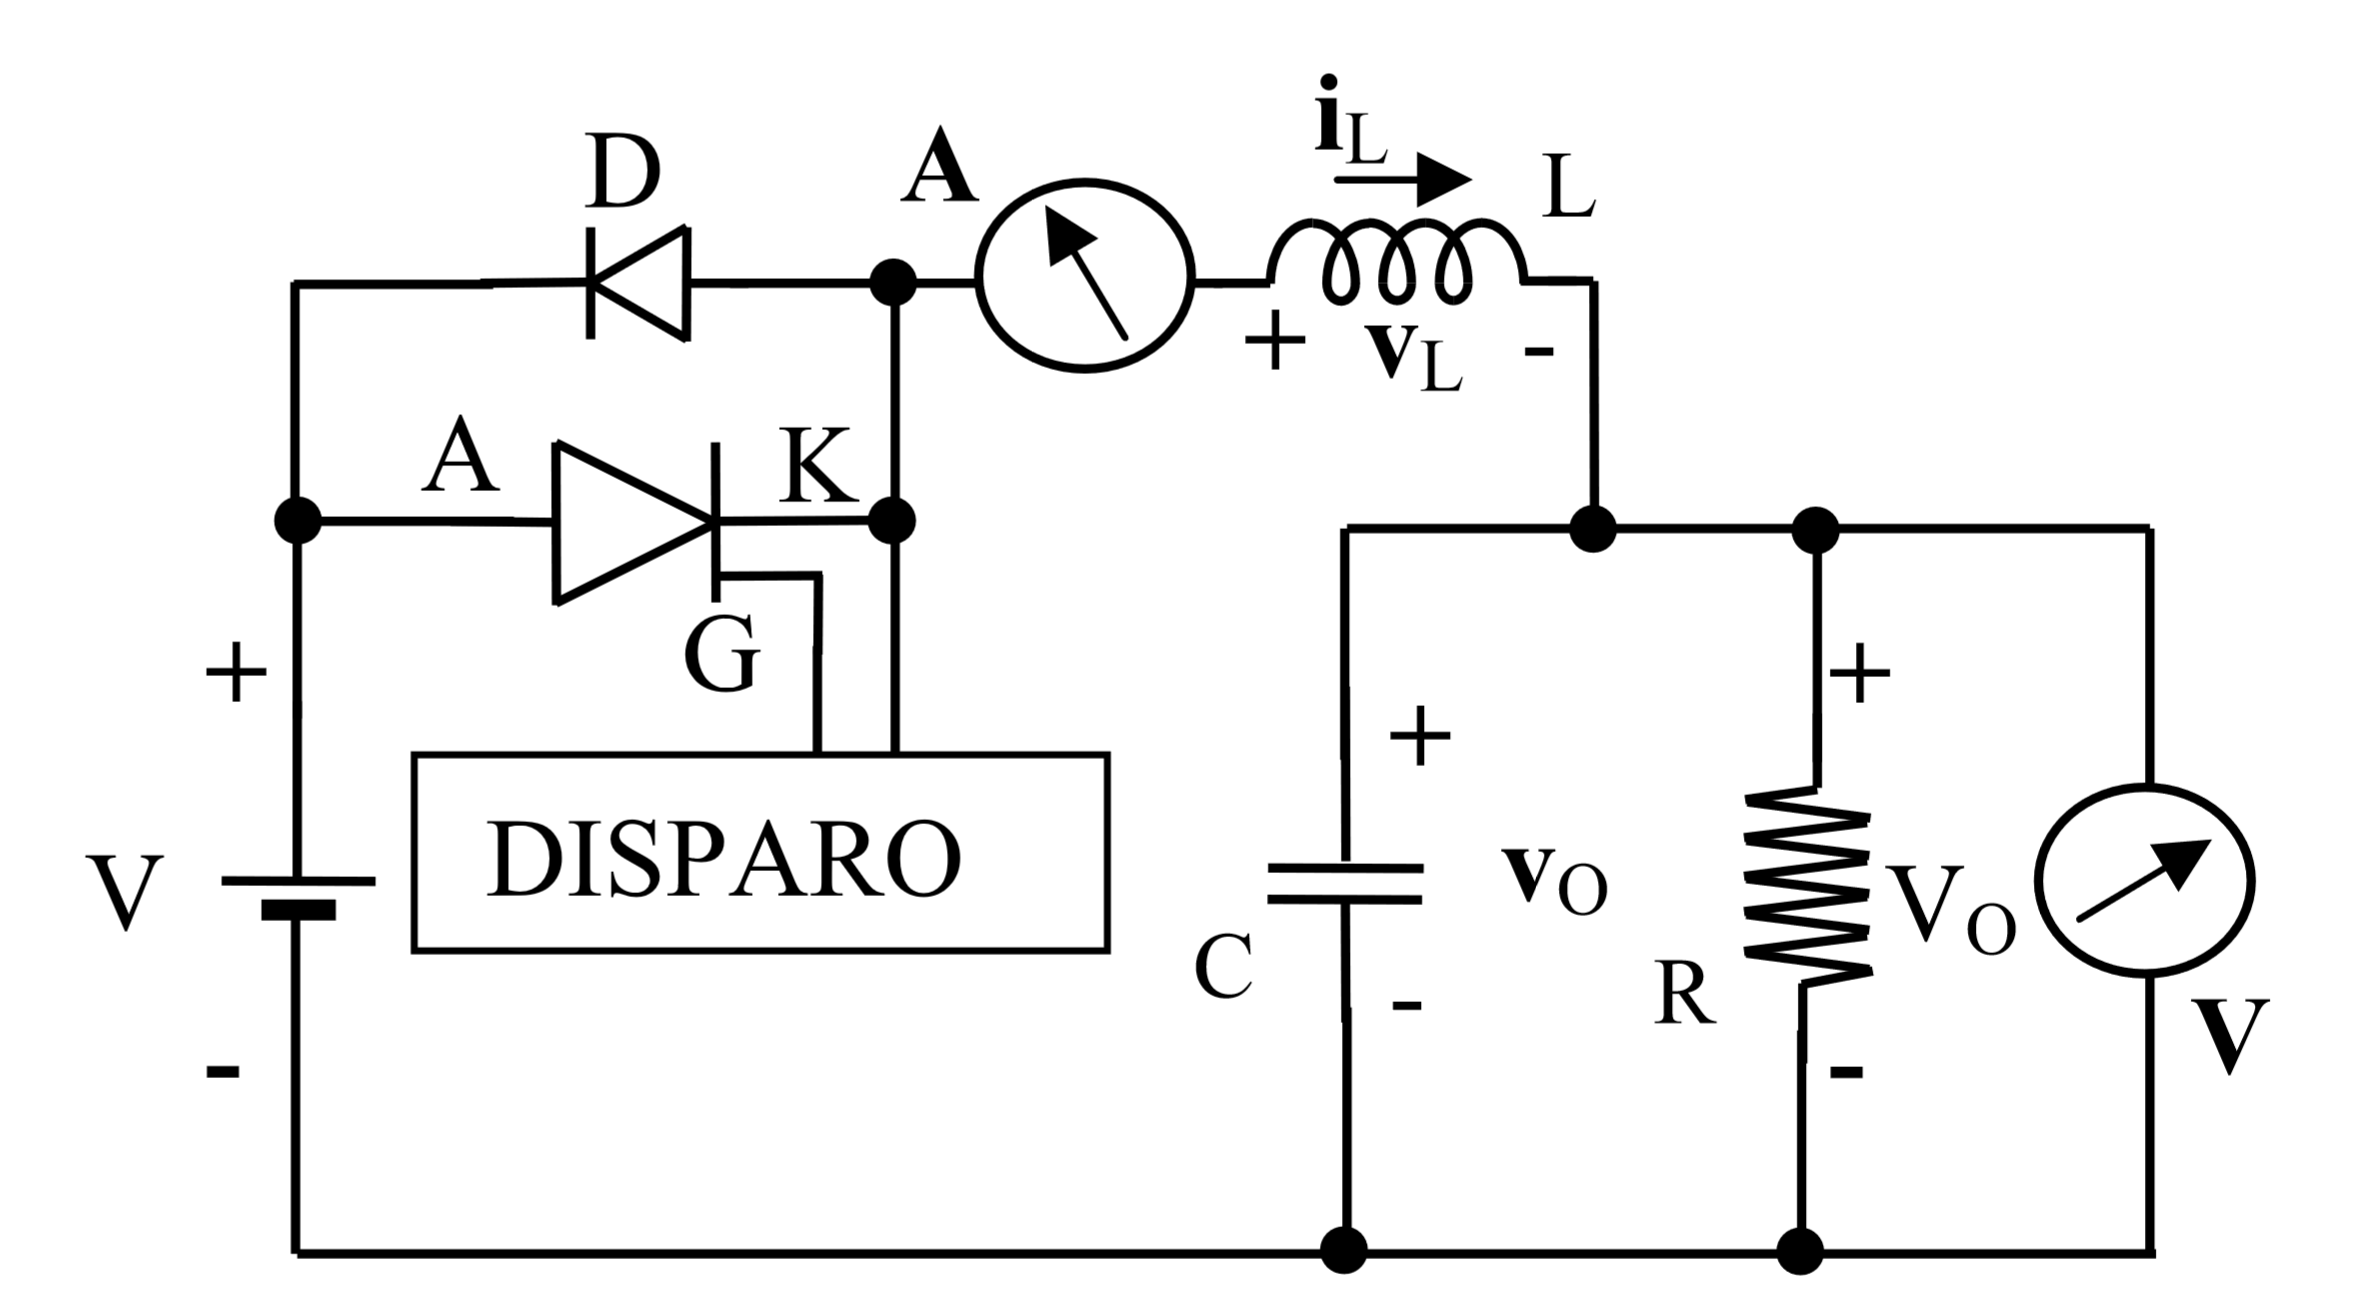
\includegraphics[keepaspectratio=true, scale=0.17]{teoricas/yes_cut}}
	\caption{Circuito de potência sem comutação do tiristor (a) e circuito de potência com comutação do tiristor por ação da carga (b).}
	\label{fig:teorica1}
	\vspace{-0.8em}
\end{figure}

No circuito da \autoref{fig:teorica1}(a), o tiristor depois de disparado não volta a passar ao corte, mesmo depois de retirado o impulso de \textit{gate}. Já no circuito da \autoref{fig:teorica1}(b) o tiristor comuta por ação da carga.

\subsubsection{Valores do voltímetro e amperímetro}

Efetuada a montagem da \autoref{fig:teorica1}(a) leram-se os valores (DC) indicados no voltímetro e amperímetro.

Regulada a fonte de alimentação para 20 V e descontando a queda de 1 V no tiristor, o valor registado na carga será de 19 V. A resistência na carga tem um valor 100 $\Omega$ e assim, de acordo com a lei de Ohm, tem-se uma corrente de 190 mA.

\subsubsection{Variações da corrente e tensão na carga em função do GI}

Verifica-se atuando no GI (em amplitude, frequência ou fator de ciclo) que não existem alterações na corrente e tensão na carga. O circuito apresentado na \autoref{fig:teorica1}(a) tem uma carga puramente resistiva e, como tal, uma vez que o tiristor começa a conduzir já não volta ao corte por variações causadas no GI.

Assim se percebe como o tiristor, uma vez que seja disparado, e tenha uma corrente de ânodo maior que a corrente de manutenção (conceito a explorar futuramente) continua a conduzir devido à realimentação positiva, mesmo que o sinal proveniente do GI seja removido. 


\subsubsection{Corrente de lançamento e corrente de manutenção}

Variando a tensão de alimentação do circuito de potência, e consequentemente a corrente na carga, determinou-se a corrente de lançamento e a corrente de manutenção.

\hspace{30mm} I\textsubscript{lançamento} = 120 mA \hspace{5mm} I\textsubscript{manutenção} = 90 mA 

A corrente de lançamento ($i_L$) corresponde à mínima corrente de ânodo necessária para manter o tiristor no estado de condução imediatamente após este ter sido disparado. Assim, uma vez que o dispositivo tenha sido ligado pelo terminal da \textit{gate} manter-se-á nesse \textit{on-state} desde que a corrente de ânodo seja maior que $i_L$.

Desde que o ânodo se mantenha polarizado positivamente, o tiristor não pode ser desligado até que a corrente de ânodo seja menor que a corrente de manutenção ($i_H$). Assim, se a corrente de ânodo for reduzida abaixo de $i_H$ o tiristor entra no estado de bloqueio, pois essa é a mínima corrente para manter o tiristor no estado de condução.

A corrente de lançamento é maior que a corrente de manutenção.

Na \autoref{fig:caracteristica} pode-se ver a característica $V\textsubscript{AK}(I)$ do tiristor, onde melhor se compreende os conceitos de corrente de lançamento e manutenção.

\pagebreak

\begin{figure}[h]
	\centering
	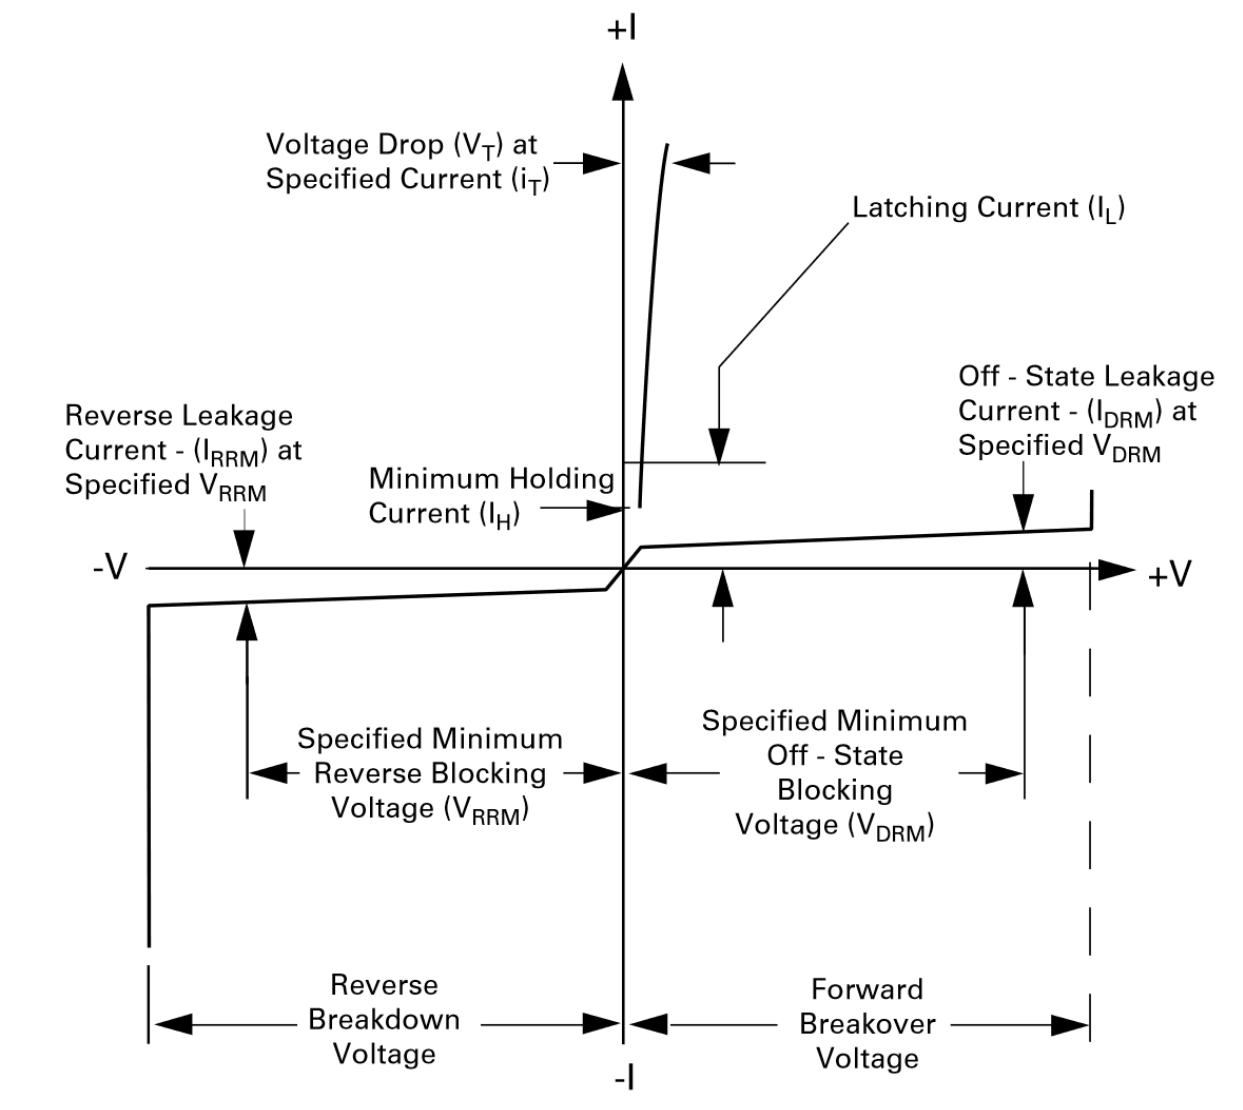
\includegraphics[keepaspectratio=true, scale=0.33]{teoricas/caracteristica}
	\caption{Característica $v(i)$ do tiristor.}
	\label{fig:caracteristica}
	\vspace{-0.8em}
\end{figure}

\subsubsection{Formas de onda da tensão no condensador e da corrente na bobine}

Nesta fase do trabalho efetua-se a montagem da \autoref{fig:teorica1}(b), colocando-se em antiparalelo com o tiristor o díodo rápido. 

A forma dos sinais de tensão no condensador e corrente na bobine podem ser observadas na \autoref{fig:imagem1}.

\begin{figure}[h]
	\centering
	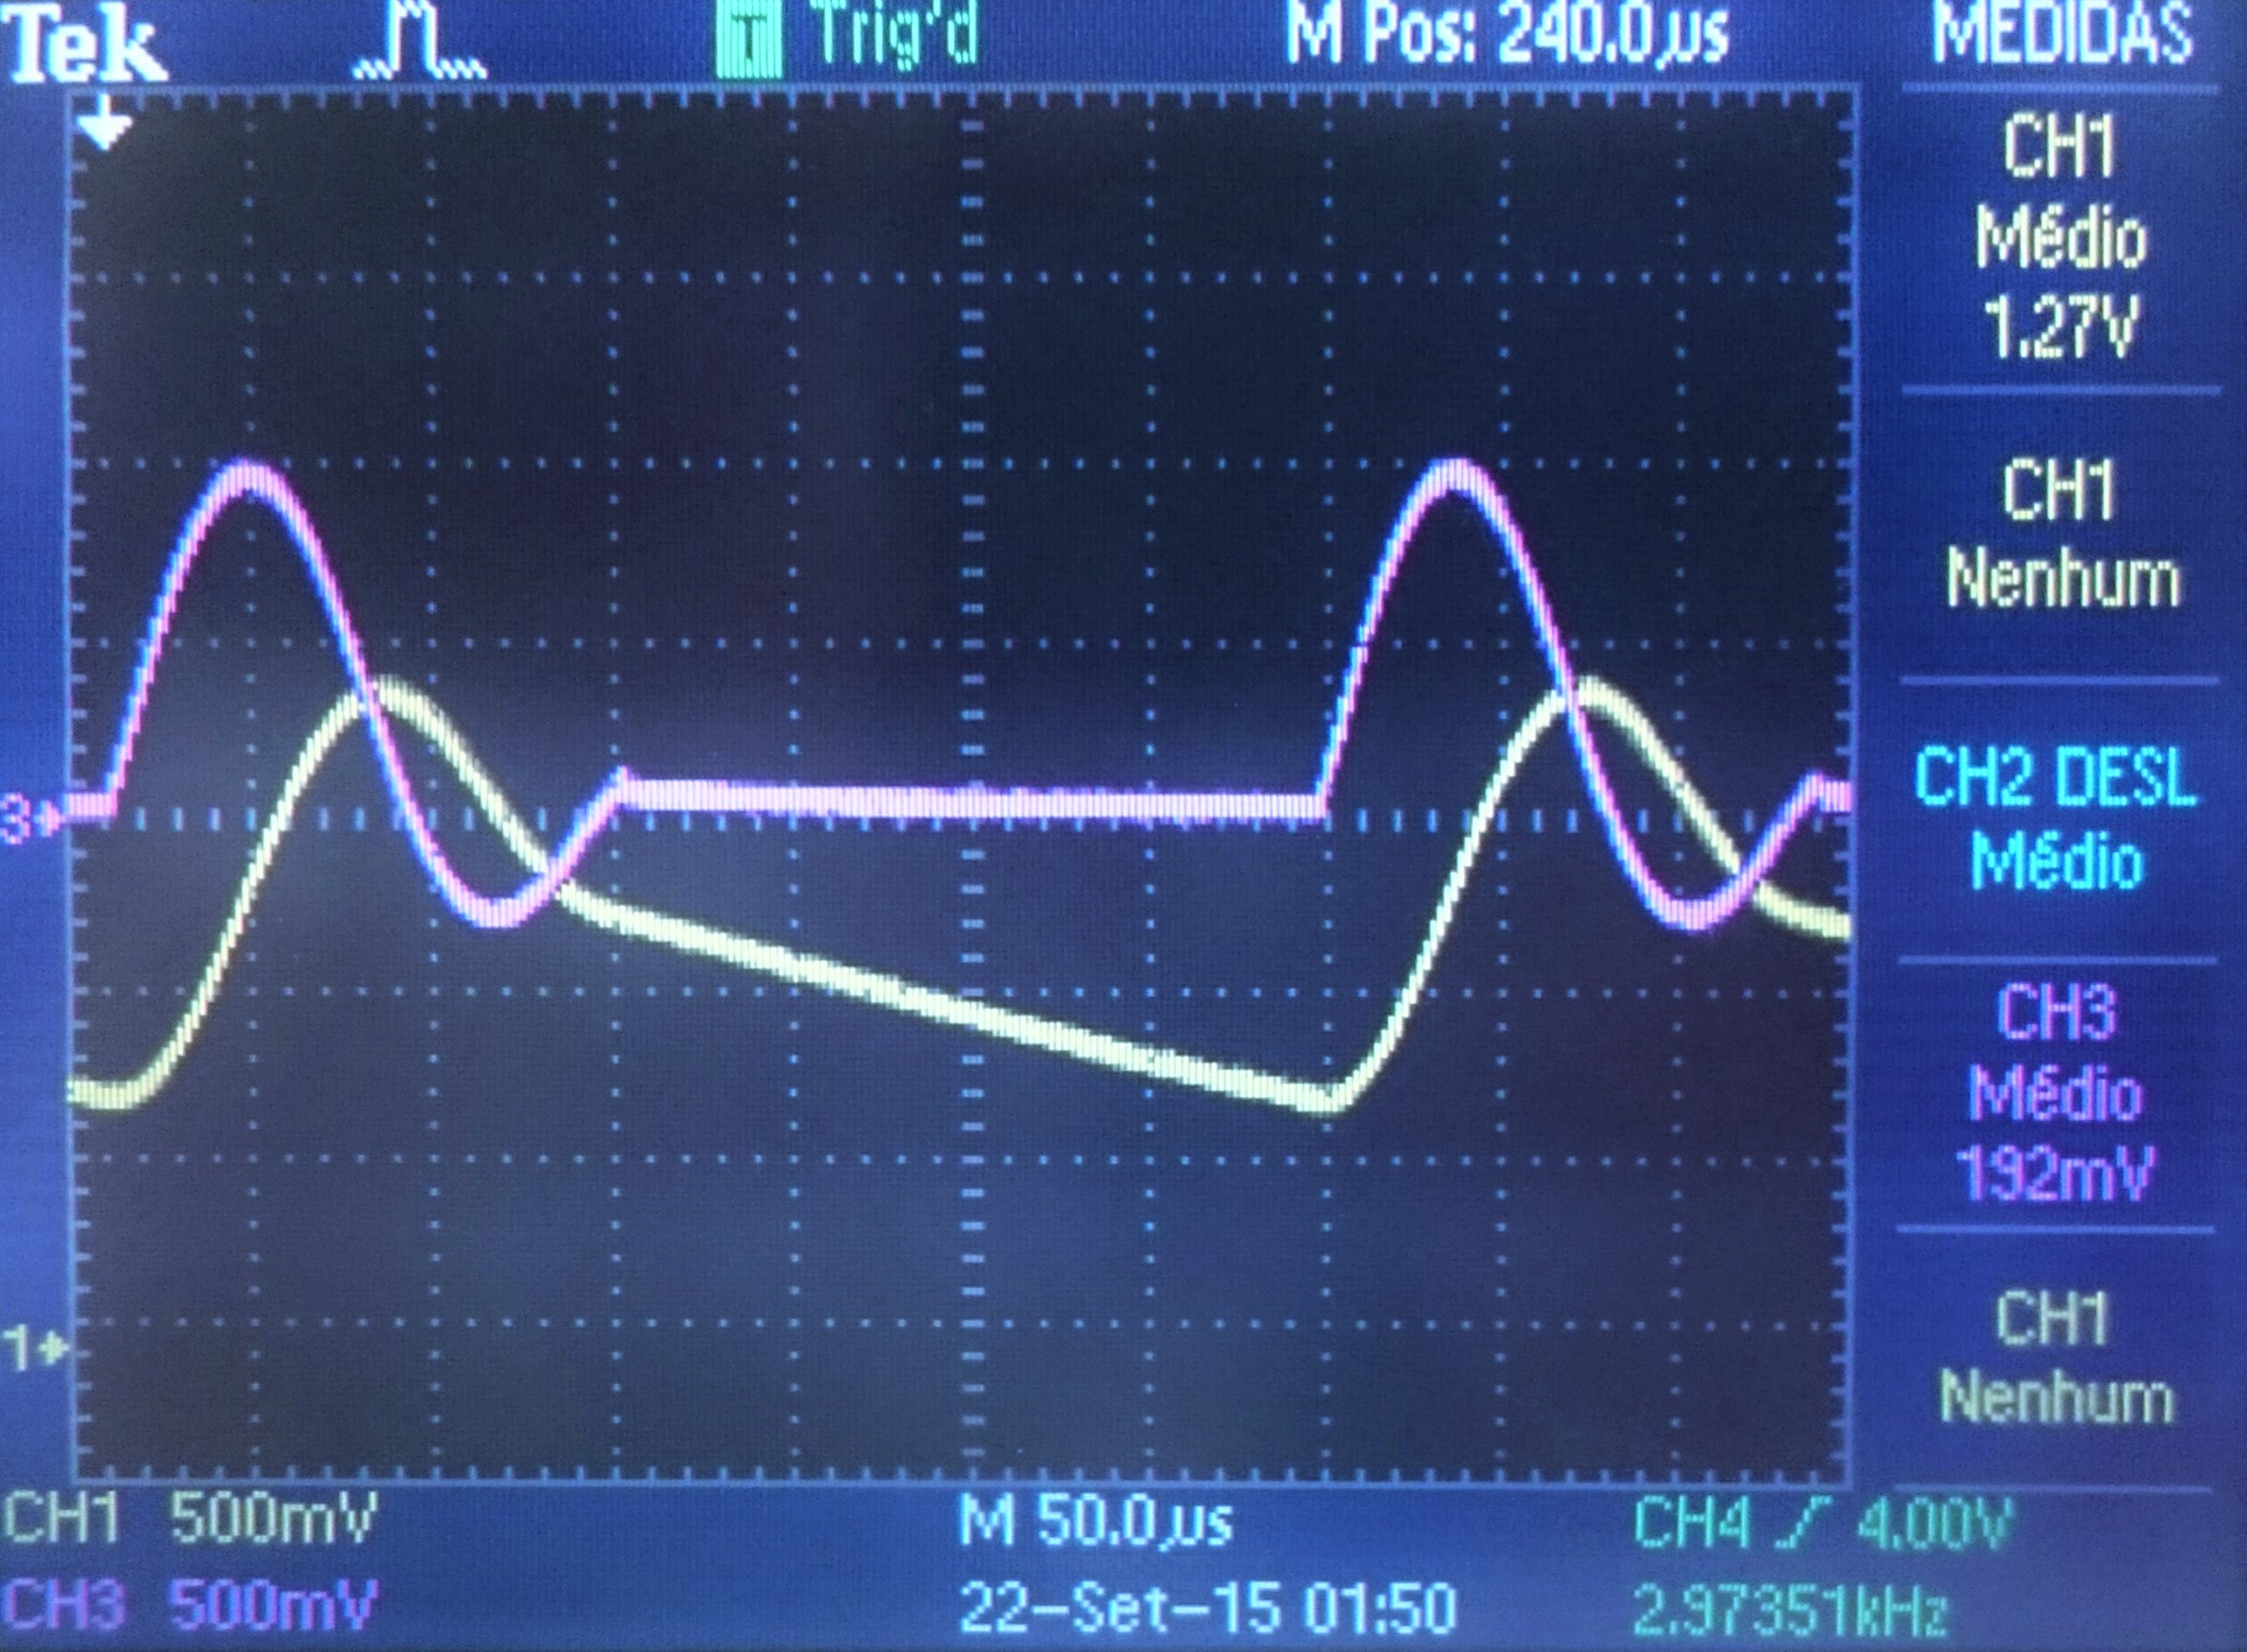
\includegraphics[keepaspectratio=true, scale=0.17]{img/imagem1}
	\caption{Tensão no condensador (a amarelo) e corrente na bobine (a rosa).}
	\label{fig:imagem1}
	\vspace{-0.8em}
\end{figure}

Como se pode verificar, no período de condução a corrente e a tensão apresentam forma sinusoidal (sinusoidal amortecida no caso da corrente). No período de corte a corrente na bobine é nula e a tensão no condensador decresce de forma exponencial, o que corresponde à sua descarga devido à resistência de carga que se encontra em paralelo com o condensador.

Também na \autoref{fig:imagem1} se pode verificar o comportamento oscilatório do circuito.

\subsubsection{Formas de onda da tensão e corrente no díodo rápido em antiparalelo}

A forma dos sinais de corrente e tensão no díodo em antiparalelo podem ser observadas na \autoref{fig:imagem2}.

\begin{figure}[h]
	\centering
	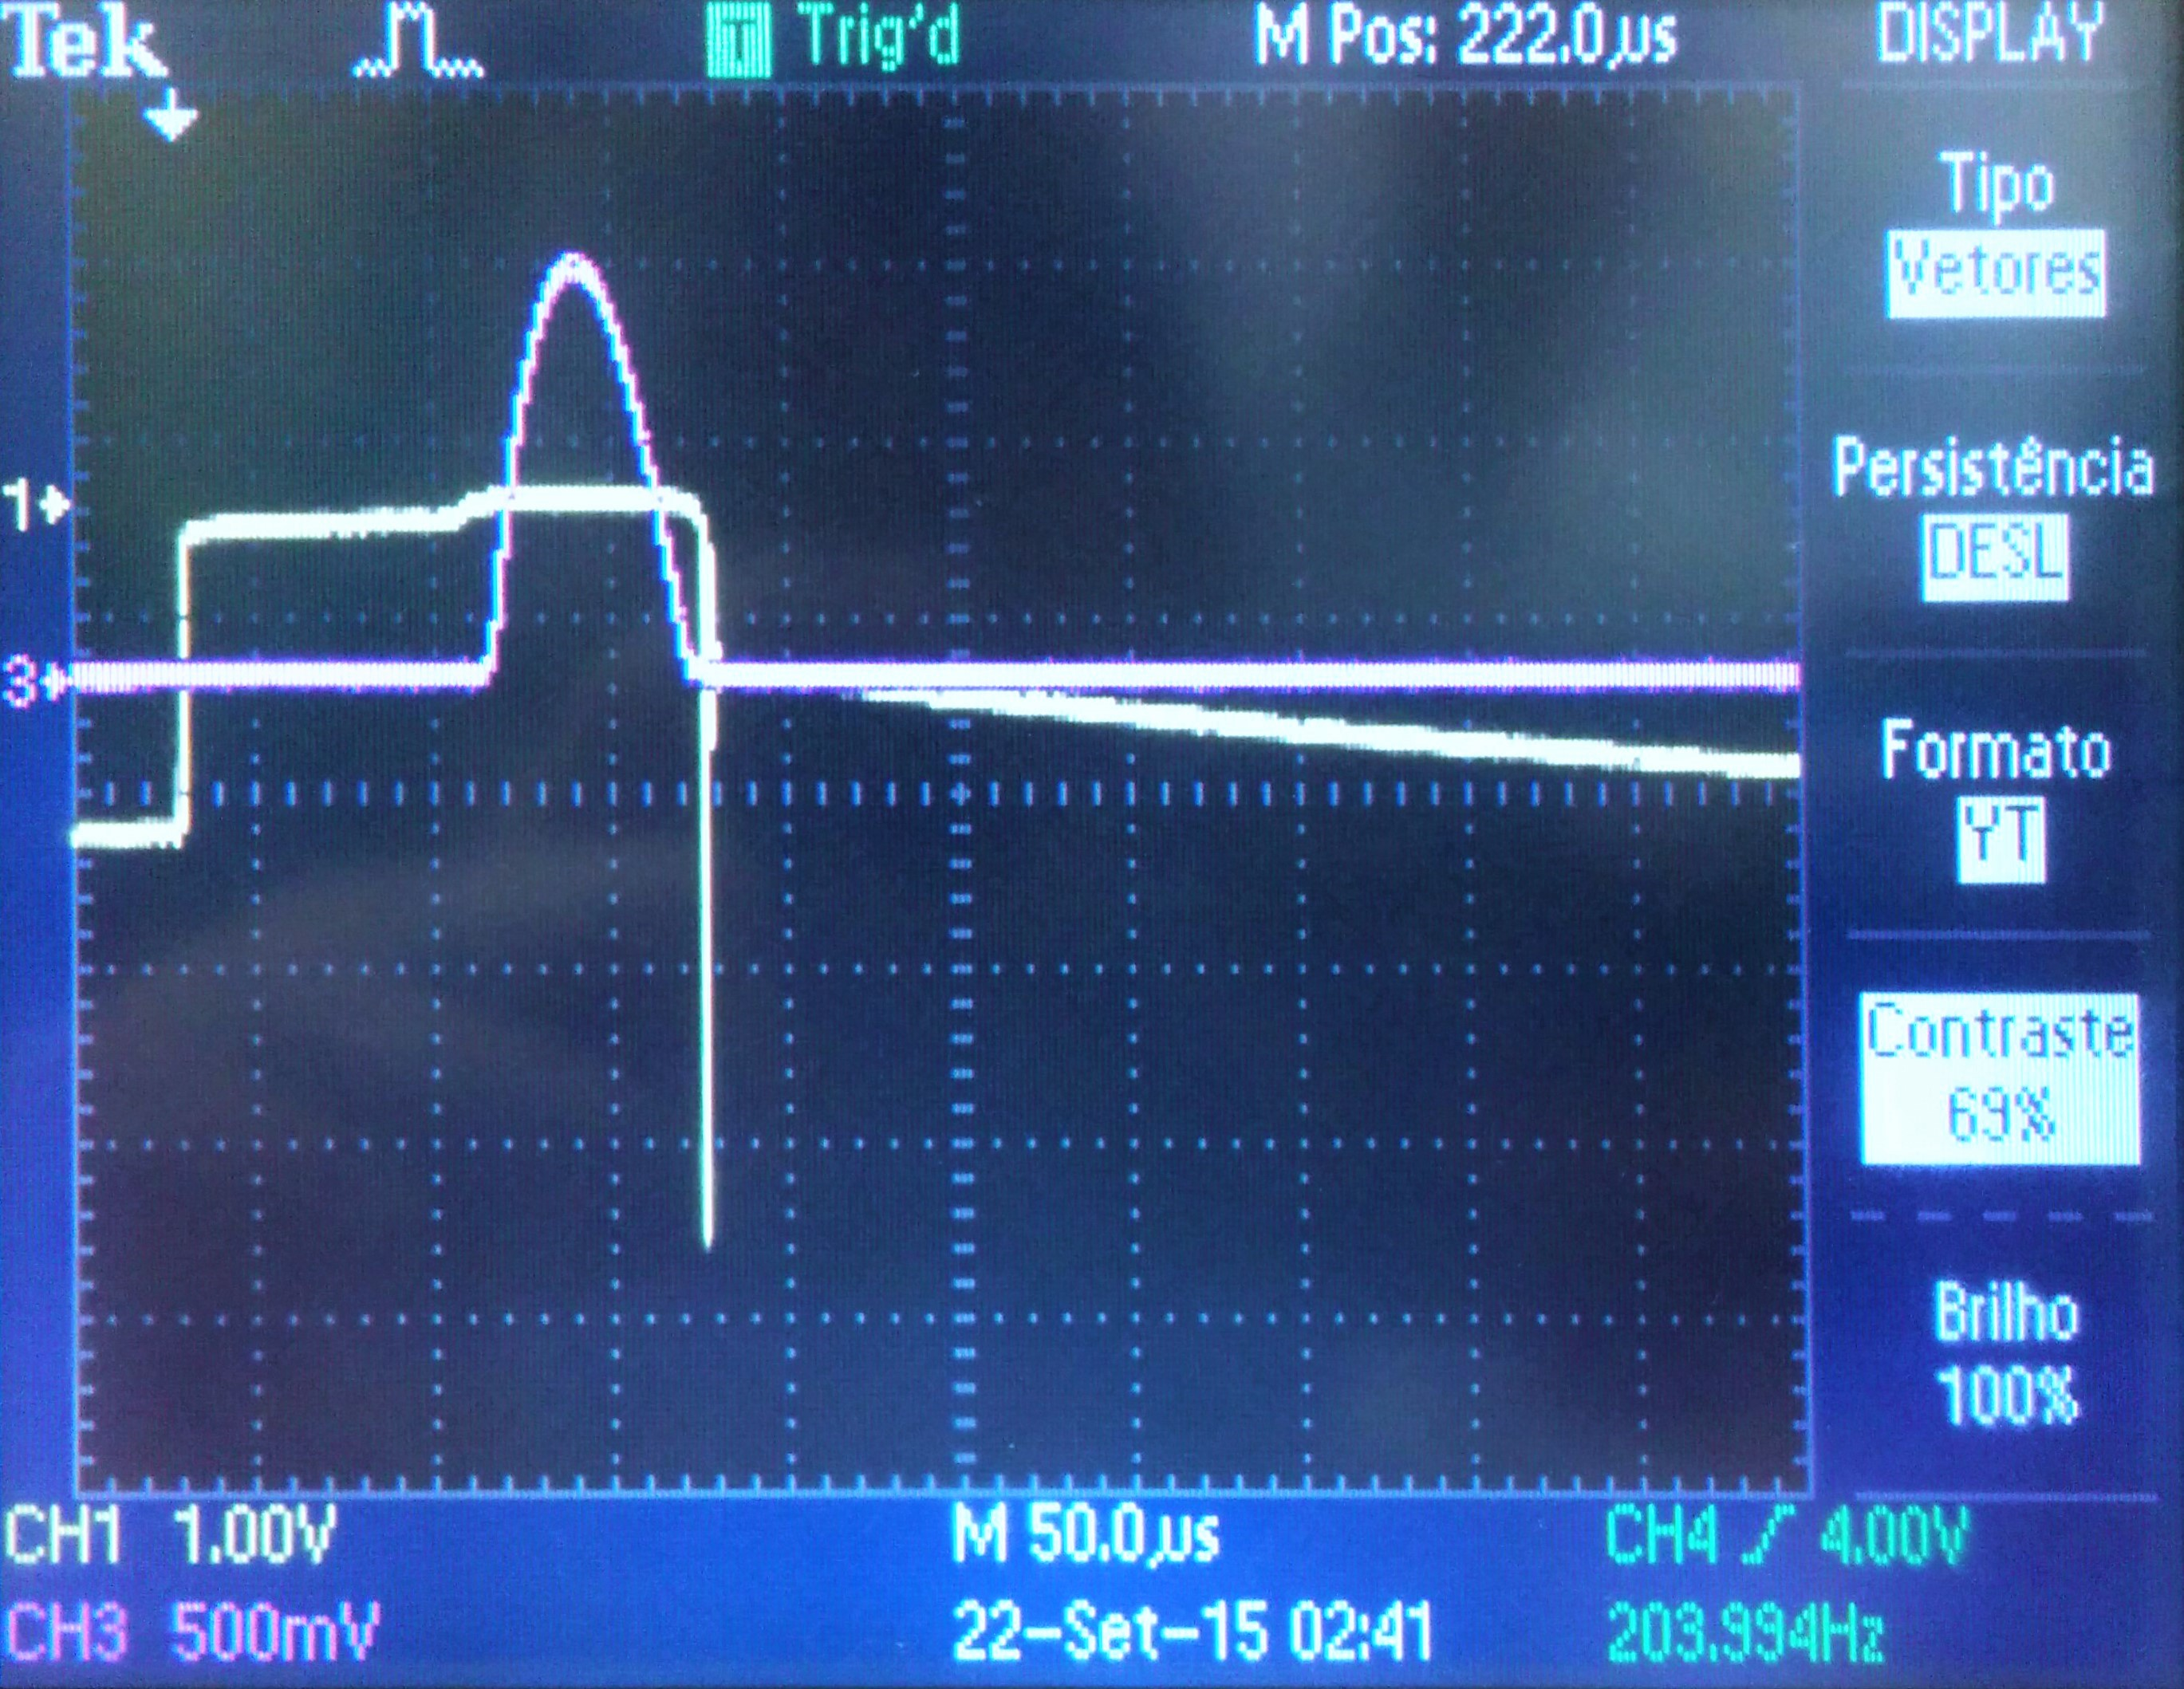
\includegraphics[keepaspectratio=true, scale=0.15]{img/imagem2}
	\caption{Tensão (a amarelo) e corrente (a rosa) no díodo rápido.}
	\label{fig:imagem2}
	\vspace{-0.8em}
\end{figure}

Nos períodos em que o tiristor conduz tem-se uma forma sinusoidal na corrente, que corresponde à alternância negativa da corrente na bobina, sendo que a tensão apresenta um valor de $1$ V aproximadamente constante, que se trata da tensão V\textsubscript{AK}. 

Já no período em que o tiristor está ao corte a corrente apresenta valor nulo, sendo o comportamento da tensão descrita em duas fases. Após o tiristor passar ao corte, a tensão observada aos terminais do díodo é V\textsubscript{AK}, que corresponde à tensão do condensador menos a de entrada. Assim que este descarrega para valores inferiores ao da tensão de entrada, aos terminais do díodo em antiparalelo ter-se-á V\textsubscript{AK}, tal como durante o período em que o tiristor está à condução.

\subsubsection{Formas de onda da tensão e corrente no tiristor}

Na \autoref{fig:imagem3} pode ver-se a tensão e corrente no tiristor.

\begin{figure}[h]
	\centering
	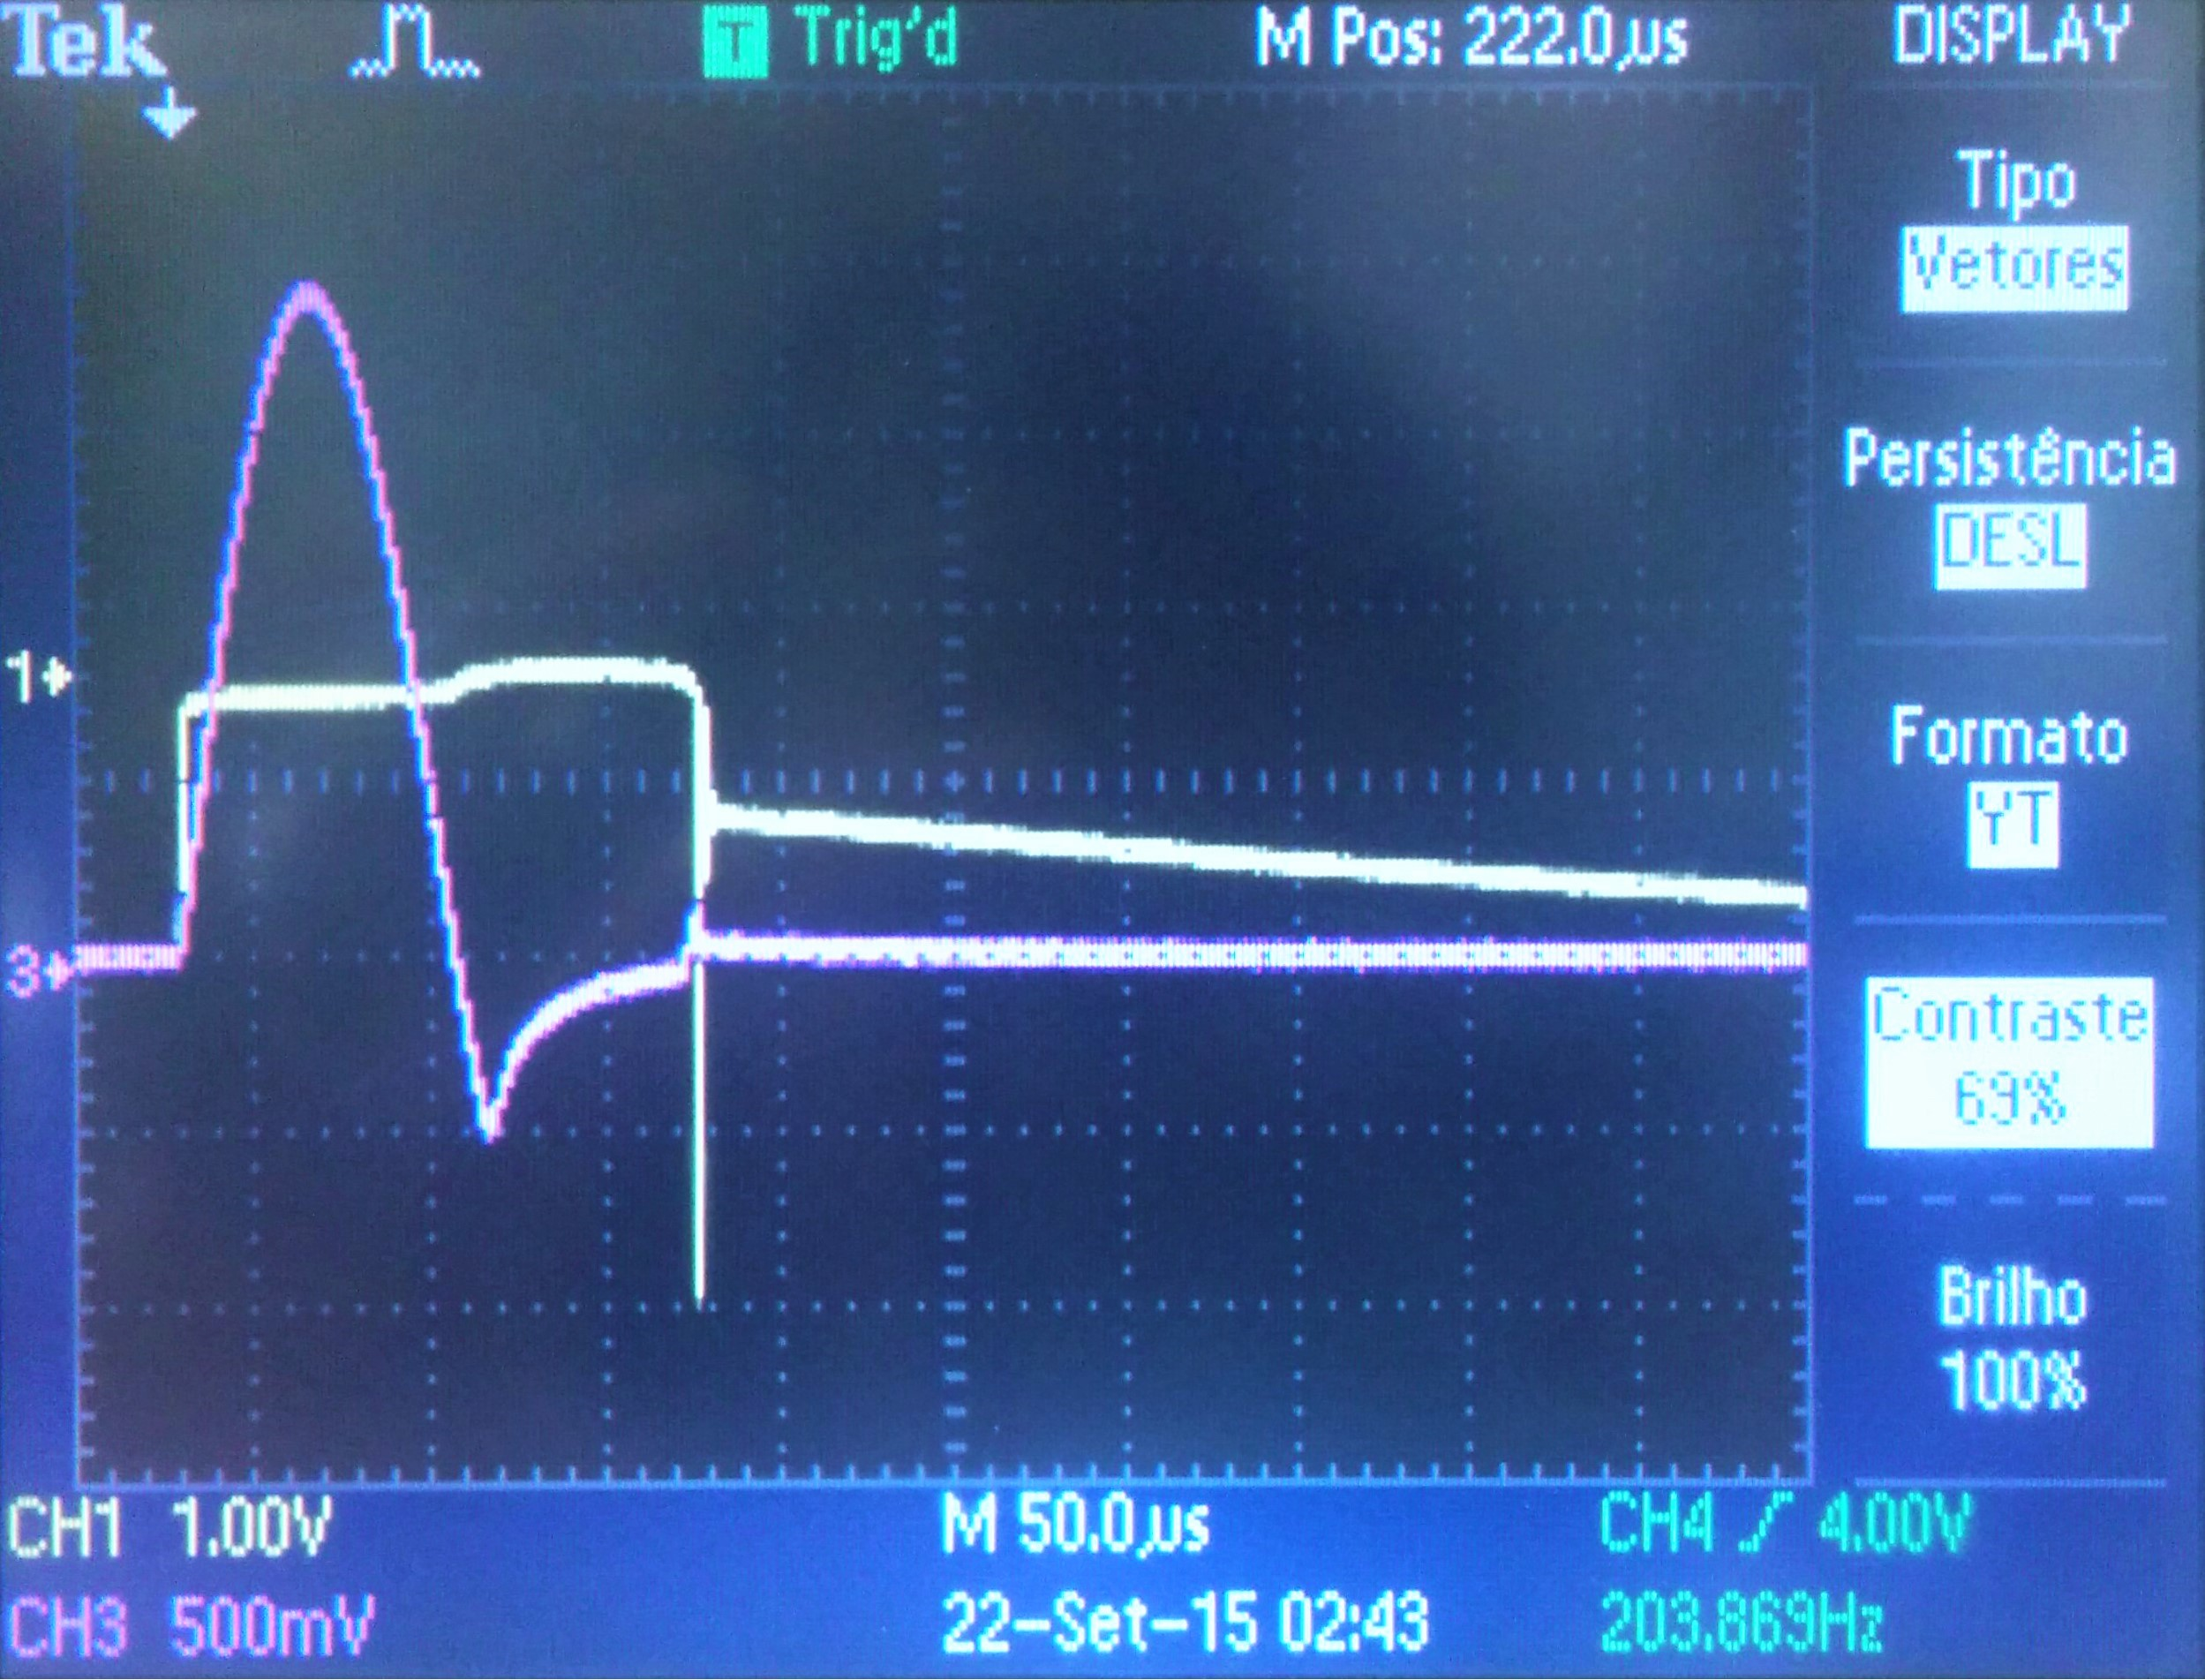
\includegraphics[keepaspectratio=true, scale=0.165]{img/imagem3}
	\caption{Tensão (a amarelo) e corrente (a rosa) no tiristor.}
	\label{fig:imagem3}
	\vspace{-0.8em}
\end{figure}


Tal como aos terminais do díodo em antiparalelo a corrente durante o período de condução do tiristor apresenta um comportamento sinusoidal, sendo neste caso o da alternância positiva da corrente na bobina, no entanto devido ao atraso da passagem ao corte do tiristor, ainda se pode observar um pouco da alternância negativa.

A tensão aos terminais do tiristor é tal como no caso da secção anterior pois ambos os dispositivos estão em paralelo.

Considera-se no entanto de interesse mencionar o pico de tensão observável em ambos os casos para momento em que o tiristor transita da condução ao corte. Isto deve-se a haver um atraso apreciável na passagem à condução do díodo e ao corte do tiristor, provocando por um instante uma derivada temporal da corrente infinita levando ao pico de tensão.


\subsubsection{Formas de onda da tensão e corrente no díodo lento em antiparalelo}

Ao utilizar o díodo lento em antiparalelo as formas de onda da corrente e tensão são as apresentadas na \autoref{fig:imagem4}.

\begin{figure}[h]
	\centering
	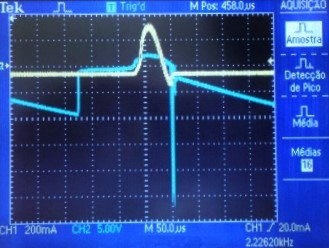
\includegraphics[keepaspectratio=true, scale=1.19]{img/imagem4}
	\caption{Tensão (a azul) e corrente (a amarelo) no diodo lento.}
	\label{fig:imagem4}
	\vspace{-0.8em}
\end{figure}

\subsubsection{Comparação entre o díodo rápido e lento}

Podem fazer-se algumas considerações ao comparar a \autoref{fig:imagem2} com a \autoref{fig:imagem4}.

Em primeiro lugar, nota-se que a tensão V\textsubscript{AK} tem um valor inferior no caso do diodo rápido. Isto deve-se a diferenças no valor da tensão de polarização direta dos dois díodos.

Também se observa que o díodo rápido tem um tempo de condução inferior, pelo que a carga perdida pelo condensador neste caso será também menor.

Por fim tem-se no caso do díodo lento um atraso no tempo de passagem à condução maior, pelo que o período em que se pode observar a arcada negativa da corrente será também maior.

\subsubsection{Funcionamento do circuito}
O funcionamento deste circuito dividi-se em três zonas, como se pode verificar na fugira seguinte:

\begin{figure}[h]
	\centering
	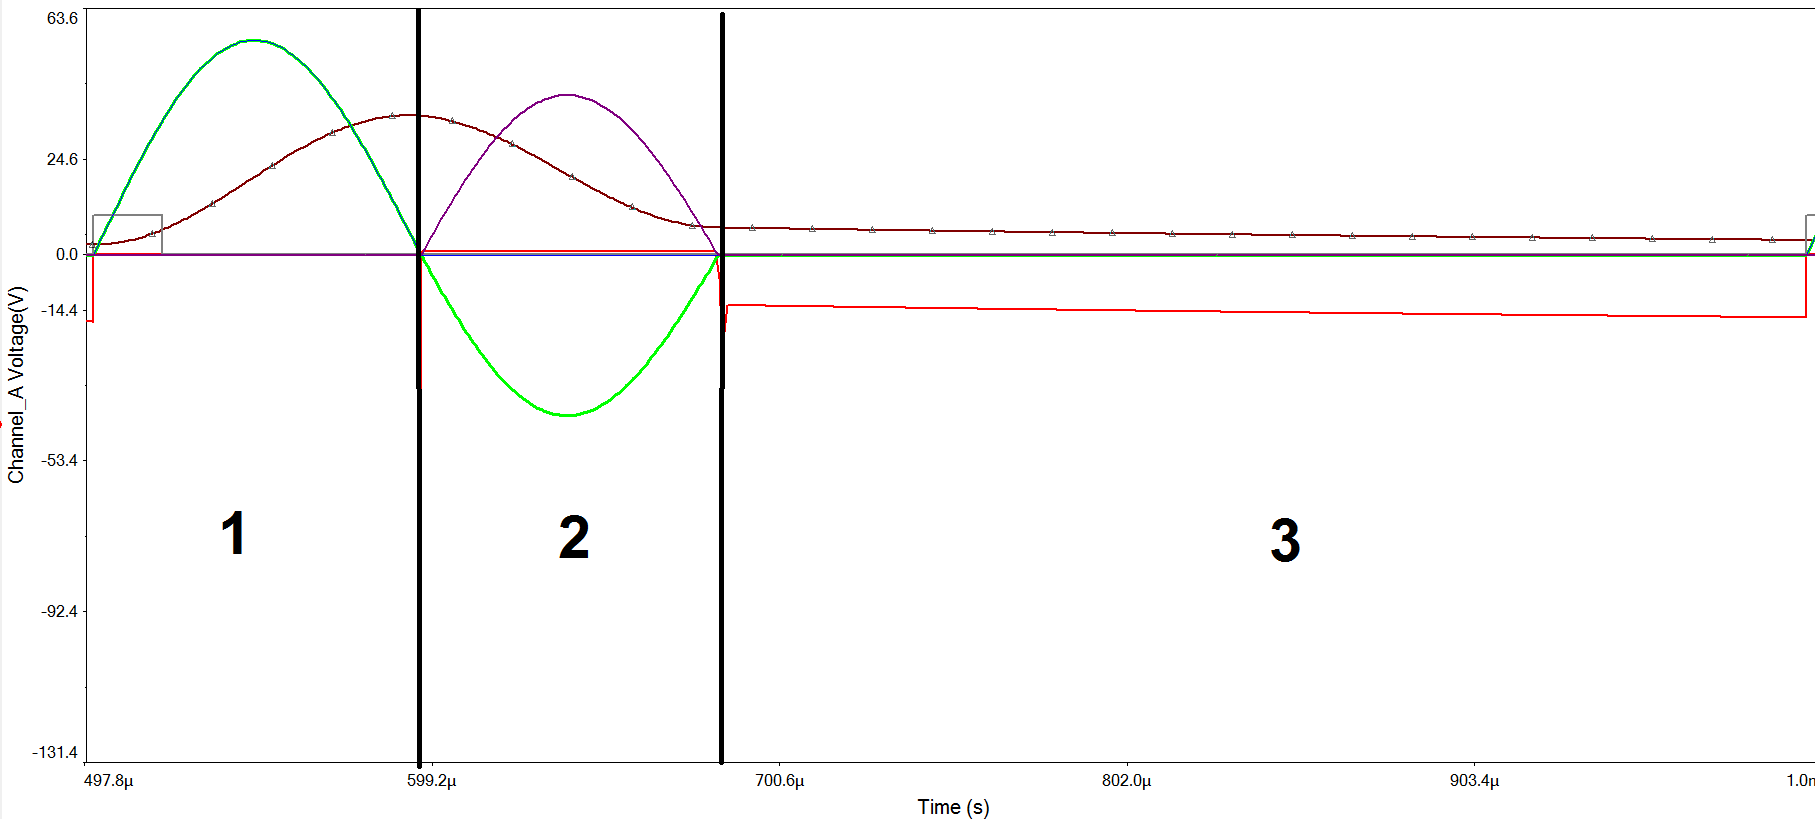
\includegraphics[keepaspectratio=true, scale=0.4]{img/funcionamento_tir}
	\caption{Resultado da simulação do circuito.}
	\label{fig:figura 1}
	\vspace{-0.8em}
\end{figure}

\subsubsection*{Zona 1}
	Zona onde o tirístor está a conduzir e o díodo ao corte.
	Analisando a simulação verifica-se que quando ocorre o impulso na \textit{gate}, sinal a cinza, a corrente no tirístor tem um comportamento imposto pela bobine, cresce até atingir o seu valor máximo e em seguida decresce até se anular, sinal a roxo. Este comportamento também influência a carga no condensador, como a corrente é no sentido da carga, este carrega até que a corrente se anula, sinal azul. Neste ponto o tirístor entra em corte.
	   
\subsubsection*{Zona 2}
	Zona onde o díodo está a conduzir e o tirístor ao corte. 
	Com a bobine carregada é necessário a sua desmagnetização, para isso coloca-se um díodo anti-paralelo com o tirístor para criar o circuito de desmagnetização. 
	Observando a simulação verifica-se que a corrente na bobine é idêntica à situação anterior mas no sentido inverso, ou seja, a desmagnetização da bobine. Com corrente a ter este comportamento é de esperar a descarga do condensador até que a corrente se anula. Neste ponto o díodo entre em corte.
	
\subsubsection*{Zona 3}
	Zona onde o díodo e o tirístor estão ao corte.
	A corrente na bobine é nula até que haja outro impulso de \textit{gate} de forma a ativar o tirístor. A tensão no condensador decresce até atingir o seu valor mínimo (período de descarga do condensador por entrega de energia à carga).
	
	Os valores máximos de corrente e tensão são determinados pelos parâmetros do circuito de disparo (período do impulso de \textit{gate}) e do circuito de potência (valores da resistência, condensador e bobine).
	A potência entregue à carga é controla através da frequência  do impulso de \textit{gate} (frequência de disparo do tirístor).




N

\subsubsection{Circuito de potência sem díodo em antiparalelo}

N

\subsubsection{Circuito de potência sem a resistência de carga}

N

\subsubsection{Expressão analítica da corrente e da tensão no condensador}

N

\pagebreak

\section{Simulação do Trabalho de Laboratório}

\subsection{Circuito de disparo}

\subsection{Circuito de potência com comutação do tiristor por acção da carga}

\pagebreak

\section{Conclusão}

\end{document}
